\documentclass[10pt,aspectratio=169
	%,handout
	]{beamer}
	\usetheme[
		sectionpages, 		% show section pages
		logo={_figures/kubernetes.png}
	]{UniNA}

	\usepackage[utf8]{inputenc}
	\usepackage[english]{babel}
	\usepackage[T1]{fontenc}

	\usepackage[scaled]{beramono}     %mono?
	\usepackage[scale=1.15]{AlegreyaSans}

	\usepackage[export]{adjustbox}
	\usepackage{csquotes}
	\usepackage[backend=biber,autocite=superscript]{biblatex}
	\addbibresource{references.bib}
	\usepackage{hyperref}

	\definecolor{kubecolor}{HTML}{326ce5}
	\definecolor{kubebg}{HTML}{1d5ce2}
	\setbeamercolor{UniNA}{bg=kubecolor}
	\setbeamercolor{frametitle}{fg=white,bg=kubecolor}

	\hypersetup{
		colorlinks,
		linkcolor=uninagray,
		citecolor=uninagray
	}

	\title[Kubernetes Overview] %shown at the top of frames
	{KUBERNETES: A Quick Walkthrough} %shown in title frame
	%\subtitle{}  % could also be a conference name

	\date{\today}

	\author[Alessandro]%shown at the top of frames
	{%shown in title frame
		Alessandro
	}

	% - Give the names in the same order as they appear in the paper.
	% - Use the \inst{?} command only if the authors have different
	%   affiliation. See the beamer manual for an example
	\institute[
		Faculty of Computer Science\\
		Free University of Bolzano\\
		Italy
	]
	{% is placed on the bottom of the title page
		Free University of Bolzano
	}

	\begin{document}

	\maketitle

	\section{Introduction}
		\subsection{What is Kubernetes?}
		\begin{frame}{Introduction}{What is Kubernetes?}
				\begin{block}{}
					Kubernetes is a portable, extensible, open-source platform for managing \textbf{containerized workloads and services}, that facilitates both \textit{declarative configuration} and \textit{automation}.\vspace{1em}
					\pause

					Kubernetes provides you with a framework to run \textbf{distributed systems} resiliently. It takes care of \textit{scaling} and \textit{failover} for your application, provides automated \textit{rollouts} and \textit{rollbacks}, \textit{storage orchestration}, and more. \autocite{kube_def}
				\end{block}
				%\pause
				%\vspace{1em}
				%\begin{columns}
				%	\begin{column}{.65\textwidth}
				%		Originally released by Google in 2015 as a successor of \textit{Borg} and \textit{Omega} \autocite{history}
				%	\end{column}
				%	\begin{column}{.25\textwidth}
				%		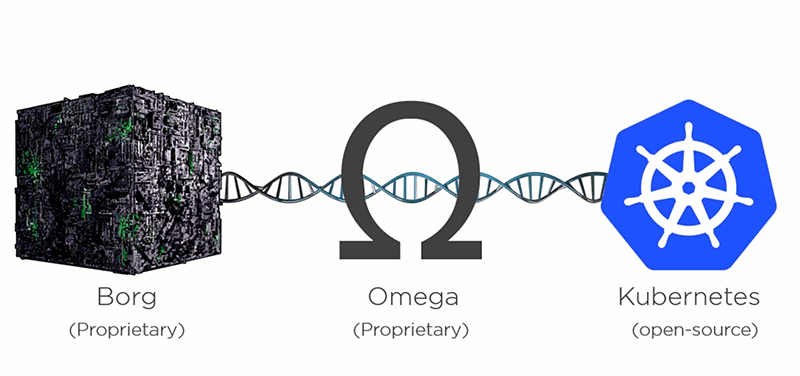
\includegraphics[width=1.2\linewidth]{images/borg-kube.png}
				%	\end{column}
				%\end{columns}
		\end{frame}

		%\subsection{Main Features}
		%\begin{frame}{Introduction}{Main Features}
		%	\begin{columns}
		%		\begin{column}{.50\textwidth}
		%			\begin{itemize}
		%				\setlength\itemsep{1em}
		%				\item Service discovery and load balancing
		%				\item Automated rollouts and rollbacks
		%				\item Self-healing
		%				\item Storage orchestration
		%				\item Secret and configuration management
		%			\end{itemize}
		%		\end{column}
		%		\begin{column}{.45\textwidth}
		%			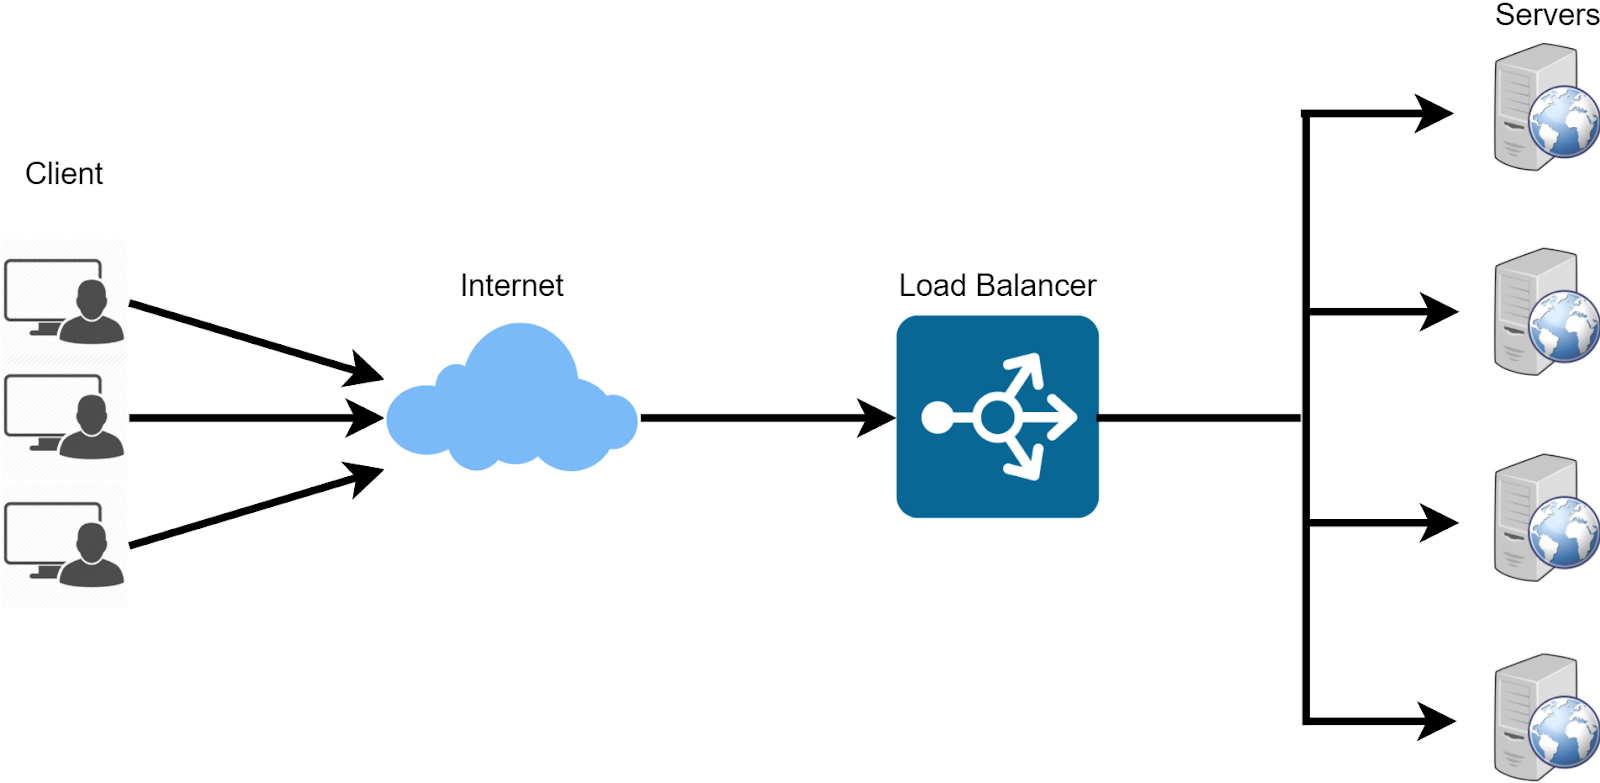
\includegraphics[width=\linewidth]{images/load-balancer.png}
		%		\end{column}
		%	\end{columns}
		%\end{frame}

	\section{Architecture}
		\subsection{Schema}
		\begin{frame}{Architecture}{Schema\autocite{kube_arch}}
			%\includegraphics<1>[width=\linewidth]{images/kube-pod.png}
			\includegraphics<1>[width=\linewidth]{images/kube-node.png}
			\includegraphics<2>[width=\linewidth]{images/kube-nodes.png}
			%\includegraphics<4>[width=\linewidth]{images/kube-control.png}
			\includegraphics<3>[width=\linewidth]{images/kube-architecture.png}
		\end{frame}

	\section{Configuration}
		\subsection{YAML Blueprint}
		\begin{frame}[fragile]{Configuration}{YAML Blueprint\autocite{kube_conf}}
			\begin{block}{deployment.yaml}
			\begin{verbatim}
			apiVersion: v1
			kind: <object>
			metadata:
			  name: <identifier>
			  labels:
			    app: <application name>
			spec:
			  <object-specific settings>
			\end{verbatim}
			\end{block}
		\end{frame}

		\subsection{Object Kinds - Stateless Application}
		\begin{frame}{Configuration}{Object Kinds - Stateless Application\autocite{kube_stateless}}
			\begin{columns}
				\begin{column}{.35\textwidth}
					\begin{itemize}
						\setlength\itemsep{1em}
						\item<1-> Pod
						\item<2-> Deployment
						\item<3-> Service
						\item<4-> HorizontalPodAutoscaler
					\end{itemize}
				\end{column}
				\begin{column}{.50\textwidth}
					\includegraphics<1>[width=.8\linewidth]{images/load-balancer-pod-t.png}
					\includegraphics<2>[width=.8\linewidth]{images/load-balancer-deployment-t.png}
					\includegraphics<3->[width=.8\linewidth]{images/load-balancer-service-t.png}
				\end{column}
			\end{columns}
		\end{frame}

		\subsubsection{Demo}
		\begin{frame}[plain,noframenumbering]
			\standoutpagelight{Demo time!}
		\end{frame}

		\subsection{Object Kinds - Stateful Application}
		\begin{frame}{Configuration}{Object Kinds - Stateful Application}
			\includegraphics<1>[width=.7\linewidth,center]{images/pv-creation.png}
			\includegraphics<2>[width=.7\linewidth,center]{images/pv-claim.png}
		\end{frame}

	\section{Conclusions}

		\subsection{Pros}
		\begin{frame}{Conclusions}{Pros}
			\begin{exampleblock}{Pros}
				\begin{itemize}
					\item Platform independent
					\item Highly customizable
					\item Quite popular
				\end{itemize}
			\end{exampleblock}
		\end{frame}

		\subsection{Usage}
		\begin{frame}{Conclusions}{Usage}
			\begin{columns}
				\begin{column}{.4\textwidth}
					\href{https://github.blog/2017-08-16-kubernetes-at-github/}{
\includegraphics[width=.33\linewidth,center]{images/logo-github.png}}
				\end{column}
				\begin{column}{.5\textwidth}
					\href{https://gc-taylor.com/blog/2019/11/21/recordings-slides-from-kubernetes-at-reddit-tales-from-production-at-kubecon-na-2019}{
\includegraphics[width=.29\linewidth,center]{images/logo-reddit.png}}
				\end{column}
			\end{columns}
			\vspace{1em}
			\pause
			\href{https://cloud.google.com/blog/products/containers-kubernetes/bringing-pokemon-go-to-life-on-google-cloud}{
\includegraphics[width=.25\linewidth,center]{images/logo-pokemon.png}}
		\end{frame}

		\subsection{Cons}
		\begin{frame}{Conclusions}{Cons}
			\begin{alertblock}{Cons}
				\begin{itemize}
					\item Overkill for small projects
					\item Requires much knowledge and expertise \textit{(helm package manager)}
					\item Documentation lacks complete examples
				\end{itemize}
			\end{alertblock}
		\end{frame}

		\subsection{End}
		\begin{frame}[plain,noframenumbering]
			\standoutpage{\bfseries\huge Thanks for your attention!}
		\end{frame}

	\begin{frame}[shrink,noframenumbering]{References}{and credits}
		Presentation theme adapted from \href{https://github.com/luistar/unina-beamer}{UniNa-Beamer}

		Kubernetes icons and diagrams from the official documentation website

		\vspace{1em}
		\textbf{Sources}
		\printbibliography[heading=none]
	\end{frame}

	\begin{frame}[plain,noframenumbering]
		\standoutpage{}
	\end{frame}
\end{document}
